\documentclass{article}
\usepackage{graphicx}
\usepackage{tikz}
\usepackage{amsmath, amssymb}
\usepackage{caption}
\usepackage[a4paper, margin=1in]{geometry} % Adjusted margins
\usepackage{parskip}
\usepackage{subcaption}
\usepackage{hyperref}
\usepackage{cleveref}
\usepackage{forest}
\usepackage{fancyhdr}
\usepackage{xcolor}  % put this in your preamble

\newcommand{\assignee}[1]{\textcolor{blue}{#1}}
\pagestyle{fancy}

\title{\textbf{Ontology and SkillGraph Documentation}}
\author{AIDF Project. PI Liu.}
\date{}
\fancyhead[L]{Limited Circulation}

\begin{document}

\maketitle
\vspace{-30pt}
\section{Requirements}
\begin{figure}[ht]
    \centering
    \includegraphics[width=1\linewidth]{images/hl_ontology.png}
    \caption{Sequential high-level ontology of the robot skill graph.}
    \label{fig:hl_ontology}
\end{figure}

In modern manufacturing, robotic assembly cells have become increasingly crucial as manufacturing systems grow more complex and autonomous. An ontology provides a standardized semantic foundation that enables seamless integration of diverse components and workflows within the assembly ecosystem. A good ontology should have the following requirements:
\begin{enumerate}
    \item (Structure) The ontology establishes a structured representation of knowledge and workflow, and a systematic approach to organize robotic algorithms. The structure should also enable the incorporation of new concepts, relationships, and capabilities as technology evolves. A good structure and clear relationship also make it accessible to non-experts, allowing them to understand and interact with complex robotic systems without deep technical expertise.
    \item (Interface) The ontology should provide a common language and interface to facilitate efficient communication between software components and robotic systems. It should also define a common language for user requirement specification. 
    \item (SkillGraph) The ontological standardization should allow for the creation of reusable skillgraphs, where domain-specific capabilities and algorithms can be mapped and composed in a modular fashion. 
    \item  (Data) Furthermore, the ontology serves as a comprehensive data management framework, enabling structured generation and organization of both operational data and associated metadata, thereby enhancing the reusability and transferability of manufacturing knowledge across different assembly scenarios and applications.
\end{enumerate}

 
\section{High-level Ontology}
\Cref{fig:hl_ontology} shows a high-level layout of our proposed ontology for robotic assembly. On a high-level, the ontology is organized sequentially into five layers and a shared layer. These layers are Task Specification, Persistent Knowledge, Decision Making, Device Abstraction, Physical Device, and the shared Data Service Layer. We break them down below.

\subsection{Task and Environment Specification}
Task and Environment specification layer defines the setup and requirements of the robotic assembly system. This can be broadly split into two categories - environment description and task specifications. Environment descriptions include multiple user-defined components, such as the description of environments, robots, objects, hardware models, calibrations, and all known environment states. The user can also define any task specification for the overall assembly cell in the form of an assembly target or sequence, as well as any operation preferences, optimization objectives, and hyperparameters. 

\subsection{Persistent Knowledge}
The Persistent Knowledge layer contains all necessary knowledge, skills, models, and domain expertise to support robot decision making. Hardware and task specifications from previous layers are passed as inputs to the skill graphs and any machine learning models. A special case is the Expert, which can be an experienced human or privileged algorithm that may control the decision making process in the next step. Other additional node that can be part of this layer can be a physics simulator or optimization solvers.


\subsection{Decision Making}
The Decision Making layer is where all robot decision-making algorithms are located and implemented in code. This layer is responsible for commanding the robot to accomplish the task. It can utilize any persistent knowledge to plan a long-horizon action plan, control the robot's behavior in real time, and estimate the state of robot and the assembly environment. The decision making layer can also be a teleoperator. Other example node that may fit this layer could be an end-to-end visual motor policy, or a collaborative human-robot decision maker.

\subsection{Device Abstraction}
The Device Abstraction layer is a standardized interface that bridges the physical device and any decision-making node. The software interface provides a standard way to communicate sensor information and robot commands to any decision-making node, which may be developed by different teams with different programming practices. The abstraction layer also ensures that the addition of new robots and new sensors can be scalable and should insulate the decision making from any complexity in managing multiple hardware devices.

\subsection{Physical Device}
The Physical Device layer represents all sensors and robots used in the assembly cell.

\subsection{Data Service}
The Data Service layer is a vertical layer designed to record and store execution data. It provides an easy-to-use utility service to log, replay, visualize, and compute the statistics of robot execution data. There are two categories of data - metadata and execution data. Metadata stores all task specifications, hardware setup, model hyperparameters, and the description of any skills or models used during the assembly process. On the other hand, execution data refer to any data generated during the decision making and execution processes. It should contain all data passing through the device abstraction layer, which can be visualized in a digital twin, saved, and replayed in future. Outputs and intermediatory statistics from decision-making nodes, such as inference time, prediction confidence, can also be recorded. 

\subsection{Plans for Implementation}
Currently, the layout of the high-level ontology remains a conceptual design. The goal is to implement key parts of the ontology to form a functional skeleton. Specifically, a skill graph, planner, and controller will be implemented. Some pre-existing individual parts, such as the robot API and data services, will be integrated. The framework will be tested first tested on Lego Assembly to ensure its correctness, then extended to other assembly tasks. On the other hand, we do not plan to implement the Expert-Teleoperate pipeline in this year's project. Still, this shows the high-level ontology is designed with the possibility of adding new components. 

For task specifications and environment description, our plan is to extend our current JSON data structure tailored to Lego assembly to more a more general format. Currently for Lego assembly, the user specifies a set of Json files, including 1) the detailed assembly sequence, 2) robot calibration and robot kinematic and, 3) existing objects in the environment and their locations. In addition to these, a more general data structure for task specification should also store the available robot tools, sensors, object type, location of CAD models, and metedata (e.g. skill hyperparameters). Before finalizing a precise definition, we will conduct more studies on potential use cases, such as the NIST box assembly testbed, and check existing ontology in the robotics community 


\section{Skill Graph}
The next sections in this documents provides a more detailed description of the skill graph within the overall proposed ontology. The skill graph serves as a centralized codebase for organizing the necessary robot- and environment-related assumptions and knowledge to enable intelligent integration and execution. The skill graph has five sections: 
\begin{enumerate}
    \item Physical Entities: \textit{Robot}, \textit{Object}, and \textit{Environment}
    
    \item Concepts: \textit{Skill}, including \textit{AtomicSkill} and \textit{MetaSkill}.
    
    \item Executables: \textit{SkillExecutor} and \textit{Algorithm}. The \textit{Algorithm} includes \textit{PlanningAlgorithm}, \textit{ControlAlgorithm}, \textit{PerceptionAlgorithm}, and \textit{Constraint Satisfaction Generator}. 

    \item Evaluation Metric: \textit{Metric}, including \textit{Constraint Evaluator}, and \textit{Condition Evaluator}.

    \item Date Structures: \textit{TaskParam}, \textit{RobotState}, and \textit{Env State}.
\end{enumerate}

Besides, we also illustrate the input to the SkillGraph, symbolized as \textit{Task}. The skill graph is demonstrated in \cref{fig:skillgraph}.
\begin{figure}[h]
    \centering
    \includegraphics[width=1\textwidth]{images/skillgraph-transbg.png}
    \caption{Symbolic Representation of Skill Graph}
    \label{fig:skillgraph}
\end{figure}

\subsection{Data Types and Relationships in Skill Graph}
There are several data types in \cref{fig:skillgraph}:
\begin{enumerate}
    \item BaseClass: \textit{Task}, \textit{Robot}, \textit{Object}, \textit{Environment}, \textit{Skill}, \textit{SkillExecutor}, \textit{Algorithm}, \textit{Metric}, \textit{TaskParam}, \textit{RobotState}, and \textit{Env State} 
    
    \item DerivedClass: \textit{AtomicSkill} and \textit{MetaSkill} are derived from baseclass \textit{Skill}. \textit{PlanningAlgorithm}, \textit{ControlAlgorithm}, \textit{PerceptionAlgorithm}, and \textit{Constraint Satisfaction Generator} are derived from baseclass \textit{Algorithm}. \textit{Constraint Evaluator} and \textit{Condition Evaluator} are derived from baseclass \textit{Metric}.
    
    \item Property: Each class might own certain properties, specified by a solid arrow with label ``prop." on it. For example, in \cref{fig:skillgraph}, \textit{atomic skills} and \textit{executor} are properties of derivedclass \textit{MetaSkill}. 
\end{enumerate}

Each data may have certain relationship with other data, and the relationships are specified by arrows. If the arrow points from A to B, indicating that A has a certain relationship with B. There are different types of arrows:
\begin{enumerate}
\item A 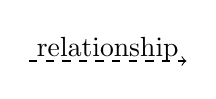
\begin{tikzpicture}[scale=0.5]
        \draw[dashed, ->] (-2,0) -- (2,0); 
        \node at (0, 0.3) {relationship};
\end{tikzpicture} B
indicates that A has certain relationship with B. For example, \underline{object library} is a vector of \textit{Object}, and \textit{Environment} is an input to \textit{SkillExecutor}.

\item A 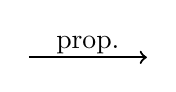
\begin{tikzpicture}[scale=0.5]
        \draw[thick, ->] (-1.5,0) -- (1.5,0); 
        \node at (0, 0.3) {prop.};
\end{tikzpicture} B
indicates that B is the property of A.
\end{enumerate}

The relationships are represented as labels on the arrows, and the relationships are defined as follows:
\begin{enumerate}
    \item A \textit{prop.} B: A has a property B. 
    \item A \textit{input to} B: A is the input to B. 
    \item A \textit{vector of} B: A is a vector of B.
    \item A \textit{type of} B: A's data type is B.
\end{enumerate}


\section{Main Components in SkillGraph}
\assignee{Peiqi}\\
The key components in the SkillGraph are:

\begin{itemize}
    \item \textbf{Skill:} Contains derived classes \textit{AtomicSkill} and \textit{MetaSkill}, which define the basic and composite robot skills.

    \item \textbf{SkillExecutor:} Defined by its four properties: \textit{function}, \textit{pre-condition}, \textit{post-condition}, and \textit{parametors}.
    
    \item \textbf{Algorithm:} Comprising derived classes \textit{PlanningAlgorithm}, \textit{ControlAlgorithm}, \textit{PerceptionAlgorithm}, and \textit{Constraint Satisfaction Genetor}.
    
    \item \textbf{Robot:} Defined by its two properties: \textit{capabilities} and \textit{robot specification}.

    \item \textbf{Object:} we allow user to define their own object type.
    
    \item \textbf{Environment:} Defined by its three properties: \textit{environment specification}, \textit{object library} and \textit{backend}.
    
    \item \textbf{Metric:} Comprising derived class \textit{Constraint Evaluator} and \textit{Condition Evaluator}.
\end{itemize}

To further enhance the structure and organization of the SkillGraph, we define several essential data structures:
\begin{itemize}
    \item \textbf{TaskParam:} Represents the parameters required for task execution, can be specified by user.
    \item \textbf{RobotState:} Captures the current state of the robot, including its joint state and end effector state.
    \item \textbf{EnvState:} Capture the environment state, including all objects' locations, and status.
\end{itemize}

Currently, our code is implemented in this \href{https://github.com/intelligent-control-lab/AIDF}{GitHub} repository. We have defined all the header files of our C++ class according to the semantics and relationships we specify below. Class implementations of all .cpp files and specific skills for Legos, are still in progress. 

In the following sections, we would give a detailed definition of each components and their relationships with other components.

\assignee{Philip for writing all the implementation details of the codes, like the pointer to the code location, and the instances of skills.}\\
\assignee{Peiqi for writing all the high-level meaning of this data structure}
\subsection{Skill}\label{sec:skills}
The \href{https://github.com/intelligent-control-lab/AIDF/blob/main/skillgraph/api/skills.hpp#L10}{Skill base class} captures the enum type, display name, optional executor, and JSON parameters for every capability exposed in the SkillGraph. Codes below 100 mark atomic skills, while identifiers from 101 upwards denote meta skills composed of atomic steps. The atomic catalogue currently covers Pick, PlaceTop, PlaceBottom, SupportBottom, SupportTop, Handover, Transit, align, Translate, Rotate, DetectPick, DetectPlace, and DetectError. Meta entries extend the same enum with PlaceWithSupport, PickAndPlace, PickAndPlaceWithSupport, PickHandoverAndPlace, PickAndPlaceRealRobot, and TranslateWithRotation.

The \href{https://github.com/intelligent-control-lab/AIDF/blob/main/skillgraph/api/skills.hpp#L58}{AtomicSkill} wrapper binds an optional target object and robot instance to a skill type and records the index of the atomic step when it is part of a meta skill. Perception-only actions use the dedicated \href{https://github.com/intelligent-control-lab/AIDF/blob/main/skillgraph/api/skills.hpp#L93}{PerceptionSkill} subclass, which stores ROS topic and launch information in a \href{https://github.com/intelligent-control-lab/AIDF/blob/main/skillgraph/api/skills.hpp#L86}{PerceptionSkillConfig}. Meta skills themselves are represented by the \href{https://github.com/intelligent-control-lab/AIDF/blob/main/skillgraph/api/skills.hpp#L118}{MetaSkill} class, which tracks the ordered atomic skill list, the robots participating in the sequence, selected objects, and the requested composition mode (temporal, functional, or spatial). String names from the JSON configuration are mapped to the enum values inside \href{https://github.com/intelligent-control-lab/AIDF/blob/main/skillgraph/src/skills.cpp#L5}{Skill::from_string}, and helper methods such as \texttt{isAtomic} and \texttt{isMeta} split the catalogue as needed.

\subsection{Skill Executor}\label{sec:skill-executor}
The execution contract is defined by the abstract \href{https://github.com/intelligent-control-lab/AIDF/blob/main/skillgraph/api/skills.hpp#L175}{SkillExecutor}. Each executor keeps copies of its pre- and post-conditions (\texttt{TaskParam}), an ordered list of algorithm implementations, and the last planned trajectory. Meta skills reuse the same interface via the \href{https://github.com/intelligent-control-lab/AIDF/blob/main/skillgraph/api/skills.hpp#L204}{MetaSkillExecutor}, which chains several atomic executors according to the requested composition type. The helper methods in \href{https://github.com/intelligent-control-lab/AIDF/blob/main/skillgraph/src/skills.cpp#L108}{skills.cpp} clone the shared pre/post conditions so downstream tasks can adjust them without mutating the original template, and \texttt{execute} remains the pure-virtual hook where concrete implementations will command the backend.

\subsection{Algorithm}\label{sec:algorithms}
The lightweight \href{https://github.com/intelligent-control-lab/AIDF/blob/main/skillgraph/api/algorithms.hpp#L14}{Algorithm} base class stores a type tag (Planning, Control, Perception) and a display name. Derived wrappers \href{https://github.com/intelligent-control-lab/AIDF/blob/main/skillgraph/api/algorithms.hpp#L32}{PlanningAlgorithm} and \href{https://github.com/intelligent-control-lab/AIDF/blob/main/skillgraph/api/algorithms.hpp#L42}{ControlAlgorithm} exist today; perception algorithms will follow the same pattern once implemented. Task-specific logic is currently provided in domain modules such as LEGO manipulation, for example the grasp generator implemented in \href{https://github.com/intelligent-control-lab/AIDF/blob/main/skillgraph/src/lego/lego_algorithms.cpp#L13}{lego_algorithms.cpp}. Executors collect whichever algorithm instances they need inside their \texttt{implementation} vector.

\subsection{Robot}
The \href{https://github.com/intelligent-control-lab/AIDF/blob/main/skillgraph/api/robots.hpp#L14}{Robot} class records the robot id, name, type, end-effector tool, degrees of freedom, capabilities, and home state. The constructor in \href{https://github.com/intelligent-control-lab/AIDF/blob/main/skillgraph/src/robots.cpp#L13}{robots.cpp} currently instantiates GP4 manipulators, computes the correct end-effector link for the left or right arm, and validates supported gripper types. Helper methods expose formatted strings for the robot and tool types and report the combined arm and hand DOF.

\subsection{Object}
The \href{https://github.com/intelligent-control-lab/AIDF/blob/main/skillgraph/api/objects.hpp#L5}{Object} struct models each manipulable workpiece. It stores the semantic type, current state (static, attached, supported, handover), owning robot, the parent link, the full pose, an optional attachment pose, and a geometric description (box, sphere, cylinder, or mesh with dimensions). Objects support deep copies through \texttt{clone}, and equality compares pose, state, and parent link contents so planners can safely copy environment states without aliasing.

\subsection{Environment}
The \href{https://github.com/intelligent-control-lab/AIDF/blob/main/skillgraph/api/environment.hpp#L16}{Environment} wrapper names each workspace, tracks whether it is a Lego or NIST task, stores the JSON specification that seeded it, and keeps the current \texttt{EnvState}. A shared pointer to a \href{https://github.com/intelligent-control-lab/AIDF/blob/main/skillgraph/api/backend.hpp#L8}{PlanInstance} backend bridges to motion-planning or simulation infrastructure. The implementation in \href{https://github.com/intelligent-control-lab/AIDF/blob/main/skillgraph/src/environment.cpp#L11}{environment.cpp} validates the environment type string and lets callers swap in different backend implementations such as the MoveIt integration.

\subsection{Metric}
Metrics are declared in \href{https://github.com/intelligent-control-lab/AIDF/blob/main/skillgraph/api/metrics.hpp#L10}{metrics.hpp}. The base \texttt{Metric} stores the evaluator name, and the derived \texttt{ConditionEvaluator} and \texttt{ConstraintEvaluator} expose boolean checks that plug into \texttt{TaskParam}. The \texttt{SmoothnessMetrics} helper struct groups trajectory quality scores (normalised jerk and directional consistency) for downstream reporting. Function bodies are placeholders today and will be extended once concrete evaluators are added.

\subsection{TaskParam}
The \href{https://github.com/intelligent-control-lab/AIDF/blob/main/skillgraph/api/tasks.hpp#L20}{TaskParam} structure collects everything an executor needs to reason about a skill: the raw JSON constraints, the list of allowed skill types, an optional target \texttt{State}, and optional algorithm hooks (\texttt{generator}, \texttt{condition_check}, \texttt{constraint_check}). Pre- and post-condition objects passed to executors are shallow copies of these structures so the planner can specialise them per skill invocation.

\subsection{State}
The multi-robot state model lives in \href{https://github.com/intelligent-control-lab/AIDF/blob/main/skillgraph/api/data_structure.hpp#L102}{data_structure.hpp}. A \texttt{State} bundles a vector of \texttt{RobotState} entries, a deep-copied \texttt{EnvState}, and the number of assembly steps already completed; equality and hashing rely on the content of each component so the planner can store states inside associative containers.

\subsection{RobotState}
Each \href{https://github.com/intelligent-control-lab/AIDF/blob/main/skillgraph/api/data_structure.hpp#L6}{RobotState} stores the robot id, MoveIt group name, joint positions, end-effector joints (\texttt{hand_values}), and an open-ended \texttt{attributes} map for extra annotations. The helper \texttt{to_string}, equality operator, and hash specialisation make the struct easy to log and compare.

\subsection{EnvState}
\href{https://github.com/intelligent-control-lab/AIDF/blob/main/skillgraph/api/data_structure.hpp#L45}{EnvState} owns deep clones of every tracked \texttt{Object}, ensuring that copies and assignments do not alias the same pointer. Equality tests compare the content of each object, and the \texttt{to_string} helper produces a human-readable dump. The global hash specialisation lets planner data structures use \texttt{EnvState} as a key.

\subsection{RobotTrajectory}
The planner expresses motion plans as \href{https://github.com/intelligent-control-lab/AIDF/blob/main/skillgraph/api/data_structure.hpp#L134}{RobotTrajectory} sequences that record the robot id, intermediate \texttt{RobotState} waypoints, timestamps, action ids, and accumulated cost. Multi-robot solutions are stored as \texttt{MRTrajectory} (a vector of per-robot trajectories).


\section{Planner}
\subsection{Domain Agnostic Task Planner}
The core planner lives in \href{https://github.com/intelligent-control-lab/AIDF/blob/main/planner/include/planner.h#L13}{AssemblyPlanner}. Its implementation (\href{https://github.com/intelligent-control-lab/AIDF/blob/main/planner/src/planner.cpp#L12}{planner.cpp}) performs a best-first search over \texttt{skillgraph::State} objects using a priority queue ordered by cumulative cost. The planner pulls the initial state from the SkillGraph, expands successors through \texttt{feasible_u} and \texttt{get_next_state}, and stops as soon as \texttt{at_target} reports success. The helper \texttt{get_path} routine backtracks the predecessor maps to recover both the state sequence and the corresponding skills once a solution is found.

\subsection{Temporal Plan Graph for Execution}
Execution scheduling is captured by the Temporal Plan Graph utilities in \href{https://github.com/intelligent-control-lab/AIDF/blob/main/planner/include/tpg.h#L1}{tpg.h}. The data structures store type-1 and type-2 edges, robot-indexed timelines, and shortcut candidates that can tighten a multi-robot schedule. The \texttt{TPG} class wraps optimisation and execution helpers for MoveIt and ROS actionlib, while the \texttt{ShortcutSampler} and \texttt{ShortcutIterator} implementations expose several shortcut heuristics that can be toggled through the \texttt{TPGConfig} parameters. These components consume the trajectories produced by the planner and hand them to the backend.

\section{Third-Party Libraries}
\subsection{lego-failure-web (Visualization)}
The web dashboard combines a ROS aggregator and a lightweight React front end to surface the status of every assembly step. The backend node in \href{https://github.com/intelligent-control-lab/AIDF/blob/main/tools/lego-failure-web/backend/failure_summary_node.py#L1}{backend/failure\_summary\_node.py} listens to pick/place classifiers, anomaly detectors, and skill executors, condenses the incoming topics into a single failure summary, and republishes the result for consumption by the UI. To give operators visual context, \href{https://github.com/intelligent-control-lab/AIDF/blob/main/tools/lego-failure-web/backend/render_assembly_steps.py#L1}{backend/render\_assembly\_steps.py} drives Blender to convert LDraw instructions into per-step GLB and PNG assets, which the React application in \href{https://github.com/intelligent-control-lab/AIDF/blob/main/tools/lego-failure-web/frontend/src/App.tsx}{frontend/src/App.tsx} displays through \texttt{@google/model-viewer}. The one-shot \href{https://github.com/intelligent-control-lab/AIDF/blob/main/tools/lego-failure-web/setup.sh}{setup.sh} script automates asset generation, ROS node launch, and frontend startup so the visualization can be brought online alongside the cell controller.

\subsection{lego-failure (Perception Skills)}
This repository hosts the perception stack that powers the DetectPick/DetectPlace skills and gap monitoring. \href{https://github.com/intelligent-control-lab/AIDF/blob/main/tools/lego-failure/scripts/pick_place_classify_node.py#L1}{scripts/pick\_place\_classify\_node.py} deploys a YOLO-based classifier that ingests the wrist camera stream (via \texttt{/robot/gen3\_image/compressed}) and publishes in-hand status to \texttt{/robot/pick\_place\_classify}. Surface quality is checked by the Detectron2 + RANSAC pipeline in \href{https://github.com/intelligent-control-lab/AIDF/blob/main/tools/lego-failure/scripts/gap_detection/lego_face_segmenter.py#L1}{scripts/gap\_detection/lego\_face\_segmenter.py}, which segments stud faces, fits contact lines, and flags structural gaps. The \href{https://github.com/intelligent-control-lab/AIDF/blob/main/tools/lego-failure/ros_scripts}{ros\_scripts} directory mirrors these utilities as ROS nodes (including bag-to-image extraction helpers), while \texttt{tools/lego-failure/models} stores the trained checkpoints that ship with the skill graph. Together, they form the perception-to-ROS bridge that our skill executors rely on during runtime.

\subsection{LegoScope (Error Detection)}
LegoScope implements the Eye-in-Finger endoscope pipeline for precise brick alignment. The main loop in \href{https://github.com/intelligent-control-lab/AIDF/blob/main/tools/LegoScope/detect_offset.py#L1}{detect\_offset.py} captures close-range images from the in-hand camera, segments LEGO studs, and refines circle fits so the detected studs lie on perpendicular tangents, yielding accurate x--y offsets and tool yaw. \href{https://github.com/intelligent-control-lab/AIDF/blob/main/tools/LegoScope/pub_detect_offset.py#L1}{pub\_detect\_offset.py} wraps this estimation into a ROS node that publishes \texttt{/tool\_offset} and \texttt{/block\_tilt}, while \href{https://github.com/intelligent-control-lab/AIDF/blob/main/tools/LegoScope/pub_camera_feed.py#L1}{pub\_camera\_feed.py} provides the compressed video stream. Detailed calibration, teleoperation guidance, and hardware notes live in \href{https://github.com/intelligent-control-lab/AIDF/blob/main/tools/LegoScope/README.md}{tools/LegoScope/README.md}, rounding out the end-to-end perception package for high-precision pick/place.

\section{Implementation Details}
In this section, we present the structure of our code and explain how each component from the previous sections is implemented within it.

\subsection{Code Structure and Component Implementation}
/AIDF \\
\textbar | config/ \\
\textbar | planner/ \\
\textbar | skillgraph/ \\
\textbar\hspace{0.45cm}\textbar | api/ (class and data structure definitions) \\
\textbar\hspace{0.45cm}\textbar\hspace{0.45cm}\textbar | Utils/ \\
\textbar\hspace{0.45cm}\textbar\hspace{0.45cm}\textbar | skillgraph.hpp (implement the structure of the skill graph)\\
\textbar\hspace{0.45cm}\textbar\hspace{0.45cm}\textbar | algorithms.hpp (implement \textit{SkillExecutor} and \textit{Algorithm}) \\
\textbar\hspace{0.45cm}\textbar\hspace{0.45cm}\textbar | backend.hpp (implement the backend definitions in \textit{Environment})\\
\textbar\hspace{0.45cm}\textbar\hspace{0.45cm}\textbar | environment.hpp (implement \textit{Environment})\\
\textbar\hspace{0.45cm}\textbar\hspace{0.45cm}\textbar | metrics.hpp (implement \textit{Metric})\\
\textbar\hspace{0.45cm}\textbar\hspace{0.45cm}\textbar | objects.hpp (implement \textit{Object})\\
\textbar\hspace{0.45cm}\textbar\hspace{0.45cm}\textbar | robots.hpp (implement \textit{Robot})\\
\textbar\hspace{0.45cm}\textbar\hspace{0.45cm}\textbar | skills.hpp (implement \textit{Skill})\\
\textbar\hspace{0.45cm}\textbar\hspace{0.45cm}\textbar | 
tasks.hpp (implement \textit{TaskParam})\\
\textbar\hspace{0.45cm}\textbar\hspace{0.45cm}\textbar | 
data\_structure.hpp (implement \textit{Data Structures})\\
\textbar\hspace{0.45cm}\textbar | src/ \\
\textbar\hspace{0.45cm}\textbar\hspace{0.45cm}\textbar | corresponding cpp files... \\
\textbar\hspace{0.45cm}\textbar | include/ \\
\textbar\hspace{0.45cm}\textbar\hspace{0.45cm}\textbar | lego/ (lego-specific implementations) \\
\textbar\hspace{0.45cm}\textbar\hspace{0.45cm}\textbar | Instance Implementation.hpp files \\
 

\end{document}
